\documentclass[10pt]{article}
\usepackage{fullpage,enumitem,amsmath,amssymb,graphicx,listings,tikz}
\setlength{\parindent}{0pt}

\begin{document}

\begin{center}
{\Large \textbf{Homework 4: Blackjack}}

\begin{tabular}{rl}
\\
Course: & CS 221 Spring 2019 \\
Name: & Bryan Yaggi
\end{tabular}
\end{center}

The search algorithms explored in the previous assignment work great when you know exactly the results of your actions. Unfortunately, the real world is not so predictable. One of the key aspects of an effective AI is the ability to reason in the face of uncertainty.
\smallskip

Markov decision processes (MDPs) can be used to formalize uncertain situations. In this homework, you will implement algorithms to find the optimal policy in these situations. You will then formalize a modified version of Blackjack as an MDP, and apply your algorithm to find the optimal policy.  

\section*{\normalsize Problem 1: Value Iteration}

In this problem, you will perform the value iteration updates manually on a very basic game just to solidify your intuitions about solving MDPs. The set of possible states in this game is $\{-2, -1, 0, 1, 2\}$. You start at state $0$, and if you reach either $-2$ or $2$, the game ends. At each state, you can take one of two actions: $\{-1, +1\}$. 
\smallskip

If you're in state $s$ and choose $-1$:
\begin{itemize}
	\item You have an 80\% chance of reaching the state $s-1$.
	\item You have a 20\% chance of reaching the state $s+1$.
\end{itemize}

If you're in state $s$ and choose $+1$:
\begin{itemize}
	\item You have an 70\% chance of reaching the state $s+1$.
	\item You have a 30\% chance of reaching the state $s-1$.
\end{itemize}

If your action results in transitioning to state $-2$, then you receive a reward of $20$. If your action results in transitioning to state $2$, then your reward is $100$. Otherwise, your reward is $-5$. Assume the discount factor $\gamma$ is $1$. 

\begin{enumerate}[label=(\alph*)]

  \item Give the value of $V_{opt}(s)$ for each state $s$ after 0, 1, and 2 iterations of value iteration. Iteration 0 just initializes all the values of $V$ to 0. Terminal states do not have any optimal policies and take on a value of 0.
  
  \item What is the resulting optimal policy $\pi_{opt}$ for all non-terminal states?
  
  \begin{center}
	  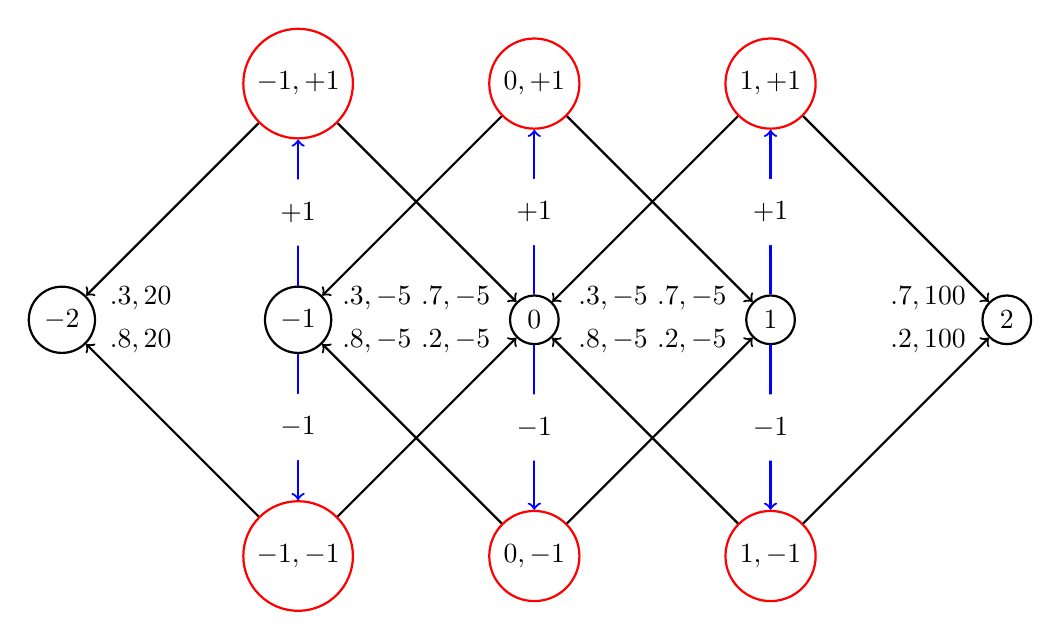
\begin{tikzpicture}
			\begin{scope}[every node/.style={circle,thick,draw}]
	    		\node (-2) at (0,0) {$-2$};
	    		\node (-1) at (3,0) {$-1$};
	    		\node (0) at (6,0) {$0$};
	    		\node (1) at (9,0) {$1$};
	    		\node (2) at (12,0) {$2$};
			\end{scope}
			\begin{scope}[every node/.style={circle,thick,draw=red}]
	    		\node (A) at (3,3) {$-1,+1$};
	    		\node (B) at (6,3) {$0,+1$};
	    		\node (C) at (9,3) {$1,+1$};
	    		\node (D) at (3,-3) {$-1,-1$};
	    		\node (E) at (6,-3) {$0,-1$};
	    		\node (F) at (9,-3) {$1,-1$};
			\end{scope}
	
			\begin{scope}[every node/.style={fill=white,circle},every edge/.style={draw=blue,thick}]
				\path [->] (-1) edge node {$+1$} (A);	    		
	    		\path [->] (0) edge node {$+1$} (B);
	    		\path [->] (1) edge node {$+1$} (C);
	    		\path [->] (-1) edge node {$-1$} (D);	    		
	    		\path [->] (0) edge node {$-1$} (E);
	    		\path [->] (1) edge node {$-1$} (F);
			\end{scope}
			\begin{scope}[every edge/.style={draw=black,thick}]
				\path [->] (A) edge node {} (0);	    		
	    		\path [->] (B) edge node {} (1);
	    		\path [->] (C) edge node {} (2);
	    		\path [->] (A) edge node {} (-2);	    		
	    		\path [->] (B) edge node {} (-1);
	    		\path [->] (C) edge node {} (0);
	    		\path [->] (D) edge node {} (-2);	    		
	    		\path [->] (E) edge node {} (-1);
	    		\path [->] (F) edge node {} (0);
	    		\path [->] (D) edge node {} (0);	    		
	    		\path [->] (E) edge node {} (1);
	    		\path [->] (F) edge node {} (2);
			\end{scope}
			\begin{scope}[]
	    		\node [above] at (1,0) {$.3,20$};
	    		\node [above] at (4,0) {$.3,-5$};
	    		\node [above] at (7,0) {$.3,-5$};
	    		\node [above] at (5,0) {$.7,-5$};
	    		\node [above] at (8,0) {$.7,-5$};
	    		\node [above] at (11,0) {$.7,100$};
	    		\node [below] at (1,0) {$.8,20$};
	    		\node [below] at (4,0) {$.8,-5$};
	    		\node [below] at (7,0) {$.8,-5$};
	    		\node [below] at (5,0) {$.2,-5$};
	    		\node [below] at (8,0) {$.2,-5$};
	    		\node [below] at (11,0) {$.2,100$};
			\end{scope}
		\end{tikzpicture}
	\end{center}
	
	$$V_{opt}^{(t)}(s) = max_{a \in actions(s)} \sum_{s'} T(s,a,s')[reward(s,a,s') + \gamma V_{opt}^{(t-1)}(s')]$$	
	
	Iteration 0:\\
	\begin{tabular}{c | c c c c c}
		$s$ & $-2$ & $-1$ & $0$ & $1$ & $2$ \\
  		$V_{opt}$ & $0$ & $0$ & $0$ & $0$ & $0$ \\
  		$\pi_{opt}$ & $none$ & $none$ & $none$ & $none$ & $none$ \\
	\end{tabular}
  
  \begin{align*}
  		V_{opt}^{(1)}(-1) &= max(.7(-5 + 1(0)) + .3(20 + 1(0)), .8(20 + 1(0)) + .2(-5 + 1(0))) = 15\\
  		V_{opt}^{(1)}(0) &= max(.7(-5 + 1(0)) + .3(-5 + 1(0)), .8(-5 + 1(0)) + .2(-5 + 1(0))) = -5\\
  		V_{opt}^{(1)}(1) &= max(.7(100 + 1(0)) + .3(-5 + 1(0)), .8(-5 + 1(0)) + .2(100 + 1(0))) = 68.5
	\end{align*}
	
	Iteration 1:\\
	\begin{tabular}{c | c c c c c}
		$s$ & $-2$ & $-1$ & $0$ & $1$ & $2$ \\
  		$V_{opt}$ & $0$ & $15.0$ & $-5.0$ & $68.5$ & $0$ \\
  		$\pi_{opt}$ & $none$ & $-1$ & $either$ & $+1$ & $none$ \\
	\end{tabular}
	
	\begin{align*}
  		V_{opt}^{(2)}(-1) &= max(.7(-5 + 1(-5)) + .3(20 + 1(0)), .8(20 + 1(0)) + .2(-5 + 1(-5))) = 14\\
  		V_{opt}^{(2)}(0) &= max(.7(-5 + 1(68.5)) + .3(-5 + 1(15)), .8(-5 + 1(15)) + .2(-5 + 1(68.5))) = 47.45\\
  		V_{opt}^{(2)}(1) &= max(.7(100 + 1(0)) + .3(-5 + 1(-5)), .8(-5 + 1(-5)) + .2(100 + 1(0))) = 67
	\end{align*}
	
	Iteration 2:\\
	\begin{tabular}{c | c c c c c}
		$s$ & $-2$ & $-1$ & $0$ & $1$ & $2$ \\
  		$V_{opt}$ & $0$ & $14.0$ & $47.45$ & $67.0$ & $0$ \\
  		$\pi_{opt}$ & $none$ & $+1$ & $+1$ & $+1$ & $none$ \\
  	\end{tabular}

\end{enumerate}
\iffalse
\section*{\normalsize Problem 2: Vowel Insertion}

Now you are given a sequence of English words with their vowels missing (A, E, I, O, and U; never Y). Your task is to place vowels back into these words in a way that maximizes sentence fluency (i.e., that minimizes sentence cost). For this task, you will use a bigram cost function.
\smallskip

You are also given a mapping \texttt{possibleFills} that maps any vowel-free word to a set of possible reconstructions (complete words). For example, \texttt{possibleFills(`fg')} returns set([`fugue', `fog']). 

\begin{enumerate}[label=(\alph*)]

  \item  Consider the following greedy-algorithm: from left to right, repeatedly pick the immediate-best vowel insertion for current vowel-free word given the insertion that was chosen for the previous vowel-free word. This algorithm does not take into account future insertions beyond the current word.

Show, as in question 1-a, that this greedy algorithm is suboptimal, by providing a realistic counter-example using English text. Make any assumptions you'd like about possibleFills and the bigram cost function, but bigram costs must remain positive.

	An example would be the input string ``Ct njys pttng dgs" for ``Cate enjoys petting dogs". ``petting" would not likely be chosen as the vowel-completed word for ``pttng" without noticing the following word is likely ``dogs".
  
  \item coding

\end{enumerate}

\section*{\normalsize Problem 3: Putting It Together}

We'll now see that it's possible to solve both of these tasks at once. This time, you are given a whitespace- and vowel-free string of alphabetical characters. Your goal is to insert spaces and vowels into this string such that the result is as fluent as possible. As in the previous task, costs are based on a bigram cost function.

\begin{enumerate}[label=(\alph*)]

  \item Consider a search problem for finding the optimal space and vowel insertions. Formalize the problem as a search problem; what are the states, actions, costs, initial state, and end test? Try to find a minimal representation of the states.
  
  The state will need to include the character index and previous verb-inserted word. The action will be the verb-inserted word created. The cost will be the bigram cost of the previous word and verb-inserted word created. The initial state will include the character index 0 and previous word \texttt{wordsegUtil.SENTENCE\_BEGIN}. The final state will be such that the character index is \texttt{len(query)}.
  
  \item coding
  
  \item  Let's find a way to speed up joint space and vowel insertion with A*. Recall that one way to find the heuristic function $h(s)$ for A* is to define a relaxed search problem $P_{rel}$ where $Cost_{rel}(s,a) \leq Cost(s,a)$ and letting $h(s)=FutureCost_{rel}(s)$.

Given a bigram model $b$ (a function that takes any $(w',w)$ and returns a number), define a unigram model $u_b$ (a function that takes any $w$ and returns a number) based on $b$. Use this function $u_b$ to help define $P_{rel}$.

One example of a $u_b$ is $u_b(w)=b(w,w)$. However this will not lead to a consistent heuristic because $Cost_{rel}(s,a)$ is not guaranteed to be less than or equal to $Cost(s,a)$ with this scheme.

Explicitly define the states, actions, cost, start state, and end state of the relaxed problem and explain why $h(s)$ is consistent.

Note: Don't confuse the $u_b$ defined here with the unigram cost function $u$ used in Problem 1.

Hint: If $u_b$ only accepts a single $w$, do we need to keep track of the previous word in our state?

	For the relaxed problem, one option is to define $u_b(w) = min (b(w', w) \mid w' \in corpus)$. $Cost_{rel} = u_b$ is guaranteed to be $\leq Cost(s,a)$ since $Cost(s,a) = b(w', w)$. The relaxed problem will be solved in reverse. The state will be the character index of query since the adjacent word is not needed to compute the relaxed cost function. The start state will be \texttt{len(query)}, and the end state will be 0. The actions will be words created. The relaxed problem will be solved to find the $FutureCost_{rel}(s)$. Then, A* can be run using $h(s) = FutureCost_{rel}(s)$.

	\item  We defined many different search techniques in class, so let's see how they relate to one another.
	
	\begin{enumerate}[label=(\arabic*)]
		\item Is UCS a special case of A*? Explain why or why not.
		
		Yes, it can be considered so because UCS is the same algorithm as A* with $h(s) = 0$.
		
		\item Is BFS a special case of UCS? Explain why or why not.	
		
		Yes, UCS would work the same as BFS for a problem where each action has the same cost and there are no cycles. UCS searches along the minimum path cost, whereas BFS searches all nodes in order by the number of hops they are from the start.
		
	\end{enumerate}

\end{enumerate}
\fi
\end{document}
